\documentclass[a4paper,12pt]{article}
\usepackage{standalone}
\usepackage{amsmath} % Package for advanced math typesetting



% Basic
\usepackage[T1]{fontenc}
\usepackage[utf8]{inputenc}
\usepackage{titlesec}
\titleformat{\section}
  {\normalfont\fontsize{14}{15}\bfseries}{\thesection}{1em}{}
\titleformat{\subsection}
  {\normalfont\fontsize{12}{15}\bfseries}{\thesubsection}{1em}{}

% Changes sections from 1.1 to 1.a
\renewcommand{\thesubsection}{\thesection.\alph{subsection}}

% ------------------------------------------------------------ %

% Packages
\RequirePackage{tcolorbox}
\usepackage{amsmath, amsthm, amssymb}
\usepackage{blindtext}
\usepackage{enumitem}
\usepackage{extramarks}
\usepackage{fancyhdr}
\usepackage[margin=1in]{geometry}
\usepackage{graphicx}
\usepackage{hyperref}
\usepackage{indentfirst}
\usepackage{listings}
\usepackage{mathrsfs}
\usepackage{mdframed}
\usepackage{multicol, multirow}
\usepackage{needspace, setspace}
\usepackage{paracol}
\usepackage{pgf, pgfplots}
\usepackage{tikz}
\usetikzlibrary{patterns}
\usepackage{silence}
\usepackage{xcolor}
\usepackage{bookmark}
\setlength{\parindent}{0pt}
\usetikzlibrary{patterns}
% \usepackage{subcaption}
\usetikzlibrary{decorations.pathreplacing}
\usepackage{caption}
\usepackage{subcaption}
\usepackage{xcolor}
\definecolor{maroon}{RGB}{128, 0, 0}
% ------------------------------------------------------------ %

% Spacings
\newcommand{\n}{\vspace{3mm}} % Context spacing
\newcommand{\s}{\vspace{1mm}} % Equation spacing
\newcommand{\m}{\vspace{-3mm}} % Reverse context spacing
\newcommand{\propdisp}{\pagebreak} % Proper display page break
\newcommand{\br}{\n\\\n}

% Wordings
\newcommand{\ans}[1][zb]{{\color{#1}\textit{Answer. }\hspace{3mm}}} % Answer
\newcommand{\arl}[1][zr]{{\color{#1}$\brr{\Leftarrow}$\hspace{3mm}}} % Left arrow
\newcommand{\arr}[1][zr]{{\color{#1}$\brr{\Rightarrow}$\hspace{3mm}}} % Right arrow
\newcommand{\cse}[2][zr]{{\color{#1}\textit{Case #2: }\hspace{1mm}}} % Case
\newcommand{\clm}[2][zr]{{\color{#1}$\vdash_{#2}$\hspace{1mm}}} % Claim
\newcommand{\prf}[1][zr]{{\color{#1}\textit{Proof. }\hspace{3mm}}} % Proof
\newcommand{\prt}[2][a]{\hspace{-2mm}{\color{#2}\textit{Part (#1) }}\hspace{1mm}} % Part
\newcommand{\prtc}[2][a]{\hspace{2mm}\prt[#1]{#2}} % Continued part

\newcommand{\rdft}[1][\sct]{{\color{zg}\textit{Definition #1}}} % Refer definition
\newcommand{\rexm}[1][\sct]{{\color{zb}\textit{Example #1}}} % Refer example
\newcommand{\rfig}[1][\sct]{{\color{zy}\textit{Figure #1}}} % Refer figure
\newcommand{\rpst}[1][\sct]{{\color{zr}\textit{Proposition #1}}} % Refer proposition
\newcommand{\rthm}[1][\sct]{{\color{zr}\textit{Theorem #1}}} % Refer theorem

\newcommand{\sct}{\thesection.\thescount} % Counter
\newcommand{\sctr}[2][0]{\the\numexpr\value{section}-#1\relax.\the\numexpr\value{scount}-#2\relax} % Relative counter

% Equations
\newcommand{\C}{\mathbb{C}} % Complex
\newcommand{\F}{\mathbb{F}} % Field
\newcommand{\I}{\mathbb{I}} % Irrational
\newcommand{\N}{\mathbb{N}} % Natural
\newcommand{\Q}{\mathbb{Q}} % Rational
\newcommand{\R}{\mathbb{R}} % Real
\newcommand{\Z}{\mathbb{Z}} % Integer

\newcommand{\GL}{\mathrm{GL}} % General linear group
\newcommand{\SL}{\mathrm{SL}} % Special linear group

\newcommand{\abs}[1]{\left| #1\right|} % Absolute
\newcommand{\bra}[1]{\left\langle #1\right\rangle} % Angled brackets
\newcommand{\brc}[1]{\left\{ #1\right\}} % Curly brackets
\newcommand{\brr}[1]{\left( #1\right)} % Round brackets
\newcommand{\brs}[1]{\left[ #1\right]} % Square brackets
\newcommand{\cond}[1]{\left. #1\right|} % Condition with right bar
\newcommand{\diff}{\,\mathrm{d}} % Differential
\newcommand{\erm}[1]{\;\;\;\;\text{#1}} % Equation remarks
\newcommand{\nrm}[1]{\left\| #1\right\|} % Norm
\newcommand{\srm}{\,\mid\,} % Set remarks

% Math operators
\let\Im\relax
\let\Re\relax

\DeclareMathOperator{\Im}{Im} % Imaginary function
\DeclareMathOperator{\Re}{Re} % Real function

% ------------------------------------------------------------ %

% Colours
\definecolor{gr}{RGB}{120, 120, 120} % Grey
\definecolor{zb}{RGB}{0, 38, 77} % Blue
\definecolor{zg}{RGB}{0, 77, 51} % Green
\definecolor{zp}{RGB}{51, 0, 77} % Purple
\definecolor{zr}{RGB}{77, 0, 38} % Red
\definecolor{zy}{RGB}{77, 64, 0} % Yellow

% Graphing
\usetikzlibrary{arrows}
\usetikzlibrary{calc}
\usetikzlibrary{patterns}
\pgfplotsset{compat=1.15}

% ------------------------------------------------------------ %

% Remark
\newcommand{\remark}[1]{
  \noindent\textbf{Remarks}
  
  \begin{nlist}
    \item Context of this document is based on university course \textit{\gettitle} from \textit{Department of Mathematics, The Chinese University of Hong Kong}. The original source can be found at \url{https://www.math.cuhk.edu.hk/course}. The author does not own the source.
    \item This document is assumed unavailable for unauthorized parties that have not attended the university course. It is prohibited to share, including distributing or copying this document to unauthorized parties in any means for any non-academic purpose.
    \item Context of this doucment may not be completely accurate. The author assumes no responsibility or liability for any errors or omissions in the context of this document.
    \item This document is under license CC-BY-SA 4.0. It is allowed to make any editions on this document, as long as terms of the license is not violated.
    #1
  \end{nlist}
}

% Prerequisites
\newenvironment{prereq}{
  \noindent \textbf{Prerequisites}\n

  This course requires prerequisites of
}{
  \n
}

% Reference list
\newenvironment{reflist}{
  \begin{alist}
    \item Course material from various professors associated to \textit{\gettitle}
}{
  \end{alist}
}

% ------------------------------------------------------------ %

% Environments
\newcounter{scount}[section] % Counter

\newenvironment{crl}{ % Corollary
  \parindent 0pt
  \begin{siderule}[linecolor=zr]{\color{zr}\textit{Corollary. }}
}{
  \end{siderule}
}

\newenvironment{cmt}{ % Comment
  \parindent 0pt
  \begin{siderule}[linecolor=zp]{\color{zp}\textit{Comment. }}
}{
  \end{siderule}
}

\newenvironment{dft}{ % Definition
  \parindent 0pt
  \refstepcounter{scount}
  \begin{siderule}[linecolor=zg]{\color{zg}\textit{Definition \sct. }}
}{
  \end{siderule}
}
\newenvironment{lem}{ % Lemma
  \parindent 0pt
  \refstepcounter{scount}
  \begin{siderule}[linecolor=zg]{\color{zg}\textit{Lemma \sct. }}
}{
  \end{siderule}
}

\newenvironment{exm}{ % Example
  \parindent 0pt
  \refstepcounter{scount}
  \begin{siderule}[linecolor=zb]{\color{zb}\textit{Example \sct. }}
}{
  \end{siderule}
}

\newenvironment{fig}{ % Figure
  \parindent 0pt
  \refstepcounter{scount}
  \begin{siderule}[linecolor=zy]{\color{zy}\textit{Figure \sct. }}\n
  
}{
  \end{siderule}
}

\newenvironment{prv}{ % Proof
  \parindent 0pt
  \begin{siderule}[linecolor=zr]\prf
}{
  \end{siderule}
}

\newenvironment{pst}{ % Proposition
  \parindent 0pt
  \refstepcounter{scount}
  \begin{siderule}[linecolor=zr]{\color{zr}\textit{Proposition \sct. }}
}{
  \end{siderule}
}

\newenvironment{tcn}{ % Technique
  \parindent 0pt
  \begin{siderule}[linecolor=zp]{\color{zp}\textit{Technique. }}
}{
  \end{siderule}
}

\newenvironment{thm}{ % Theorem
  \parindent 0pt
  \refstepcounter{scount}
  \begin{siderule}[linecolor=zr]{\color{zr}\textit{Sætning \sct. }}
}{
  \end{siderule}
}

\newenvironment{rmatrix}{ % Matrix in round brackets
  \left(\begin{matrix}
}{
  \end{matrix}\right)
}

\newenvironment{alist}{ % Alphabetical list
  \begin{enumerate}[label=(\alph*)]
}{
  \end{enumerate}
}

\newenvironment{Alist}{ % Capitalized alphabetical list
  \begin{enumerate}[label=(\Alph*)]
}{
  \end{enumerate}
}

\newenvironment{nlist}{ % Number list
  \begin{enumerate}[label=(\arabic*)]
}{
  \end{enumerate}
}

\newenvironment{plist}{ % Point list
  \begin{itemize}
}{
  \end{itemize}
}

\newenvironment{rlist}{ % Roman list
  \begin{enumerate}[label=(\roman*)]
}{
  \end{enumerate}
}

\newmdenv[ % Siderule line
  topline=false,
  bottomline=false,
  rightline=false,
  rightmargin=0
]{siderule}


% ------------------------------------------------------------ %
% Warning filters
\WarningFilter{mdframed}{You got a bad break}
\hfuzz=8pt


% Load required packages
\usepackage{tcolorbox}
% ------------------------------------------------------------ %

% Code

\usepackage{amsmath}
\usepackage{graphicx}
\definecolor{bluekeywords}{rgb}{0.13,0.13,1}
\definecolor{greencomments}{rgb}{0,0.5,0}
\definecolor{redstrings}{rgb}{0.9,0,0}
\definecolor{bgcolor}{rgb}{0.95,0.94,0.94}
\usepackage{listings}
\usepackage{upquote}
\usepackage{xcolor}

\lstdefinelanguage{Python}
{
  keywords={typeof, null, catch, switch, in, int, str, float, self},
  keywordstyle=\color{ForestGreen}\bfseries,
  ndkeywords={boolean, throw, import},
  ndkeywords={return, class, if ,elif, endif, while, do, else, True, False , catch, def},
  ndkeywordstyle=\color{BrickRed}\bfseries,
  identifierstyle=\color{black},
  sensitive=false,
  comment=[l]{\#},
  morecomment=[s]{/*}{*/},
  commentstyle=\color{purple}\ttfamily,
  stringstyle=\color{red}\ttfamily,
}

\lstset
{ %Formatting for code in appendix
    language=Python,
    numbers=left,
    stepnumber=1,
    showstringspaces=false,
    tabsize=1,
    breaklines=true,
    breakatwhitespace=false,
    backgroundcolor=\color{bgcolor},  % Background color
    basicstyle=\ttfamily\footnotesize, % Code font size and style
    frame=single,                    % Adds a frame around the code
    rulecolor=\color{bgcolor},       % Frame color
    breaklines=true,                 % Breaks long lines
}
 % Assuming these files exist and are correctly referenced
\graphicspath{ {../../pictures/IDMA/IDMA2a}} % Assuming a pictures folder has been made and is correctly referenced

% \renewcommand{\thesection}{5.\arabic{section}} % Substitue 5. for any number

% Changes sections from 1.1 to 1.a
\renewcommand{\thesubsection}{\thesection.\alph{subsection}}

\begin{document}
% \includepdf[pages=-]{../../pictures/forside}

\title{Københavns Universitet\\
Introduktion til diskret matematik og algoritmer - Problem set 2}
\author{Victor Vangkilde Jørgensen}
\makeatletter
\let\getauthor\@author
\let\gettitle\@title
\makeatother
\maketitle
\thispagestyle{empty}
\n\n
 % Assuming this file contains the cover page setup

\pagebreak
\pagestyle{empty}
\tableofcontents
\pagebreak
\pagestyle{fancy}
\fancyhf{}
\setlength{\headheight}{15.2pt}
\renewcommand{\footrulewidth}{0.4pt}
% \fancyhead[R]{\nouppercase \lastrightmark}
\fancyfoot[L]{\gettitle}
\fancyfoot[R]{\thepage}
 % Assuming this file contains the header setup
\maketitle % This command will actually insert the title into the document

\section[Question 1]{Question 1 - In this problem we wish to compare different sorting algorithms.}

\subsection[]{The exercises in Chapter 2 of CLRS mention the bubblesort algorithm, which can be further optimized as follows:}
\begin{lstlisting}
OptimizedBubbleSort (A)
    i := 1
    swapped := true
    while (i <= size(A) and swapped) {
        swapped := false
        for j := 1 upto size(A) - i {
            if (A[j] > A[j + 1]) {
                tmp := A[j]
                A[j] := A[j + 1]
                A[j + 1] := tmp
                swapped := true
            }
        }
        i := i + 1
    }
\end{lstlisting}
\begin{itemize}
    \item [] \textbf{Run the optimized bubblesort algorithm by hand on the array}
    \item [] \textbf{A = [5, 2, 19, 7, 6, 12, 10, 17, 13, 14]}
    \item [] \textbf{and show how the elements in the array are moved (similarly to what was done for insertion sort in class). Argue formally why this algorithm is guaranteed to always sort an array correctly. Analyse the time complexity of the algorithm.}
    \item [] \textbf{Hint: Try to find a nice invariant for the inner while loop to help you argue correctness.}
\end{itemize}

\begin{figure}[h] 
    \centering
    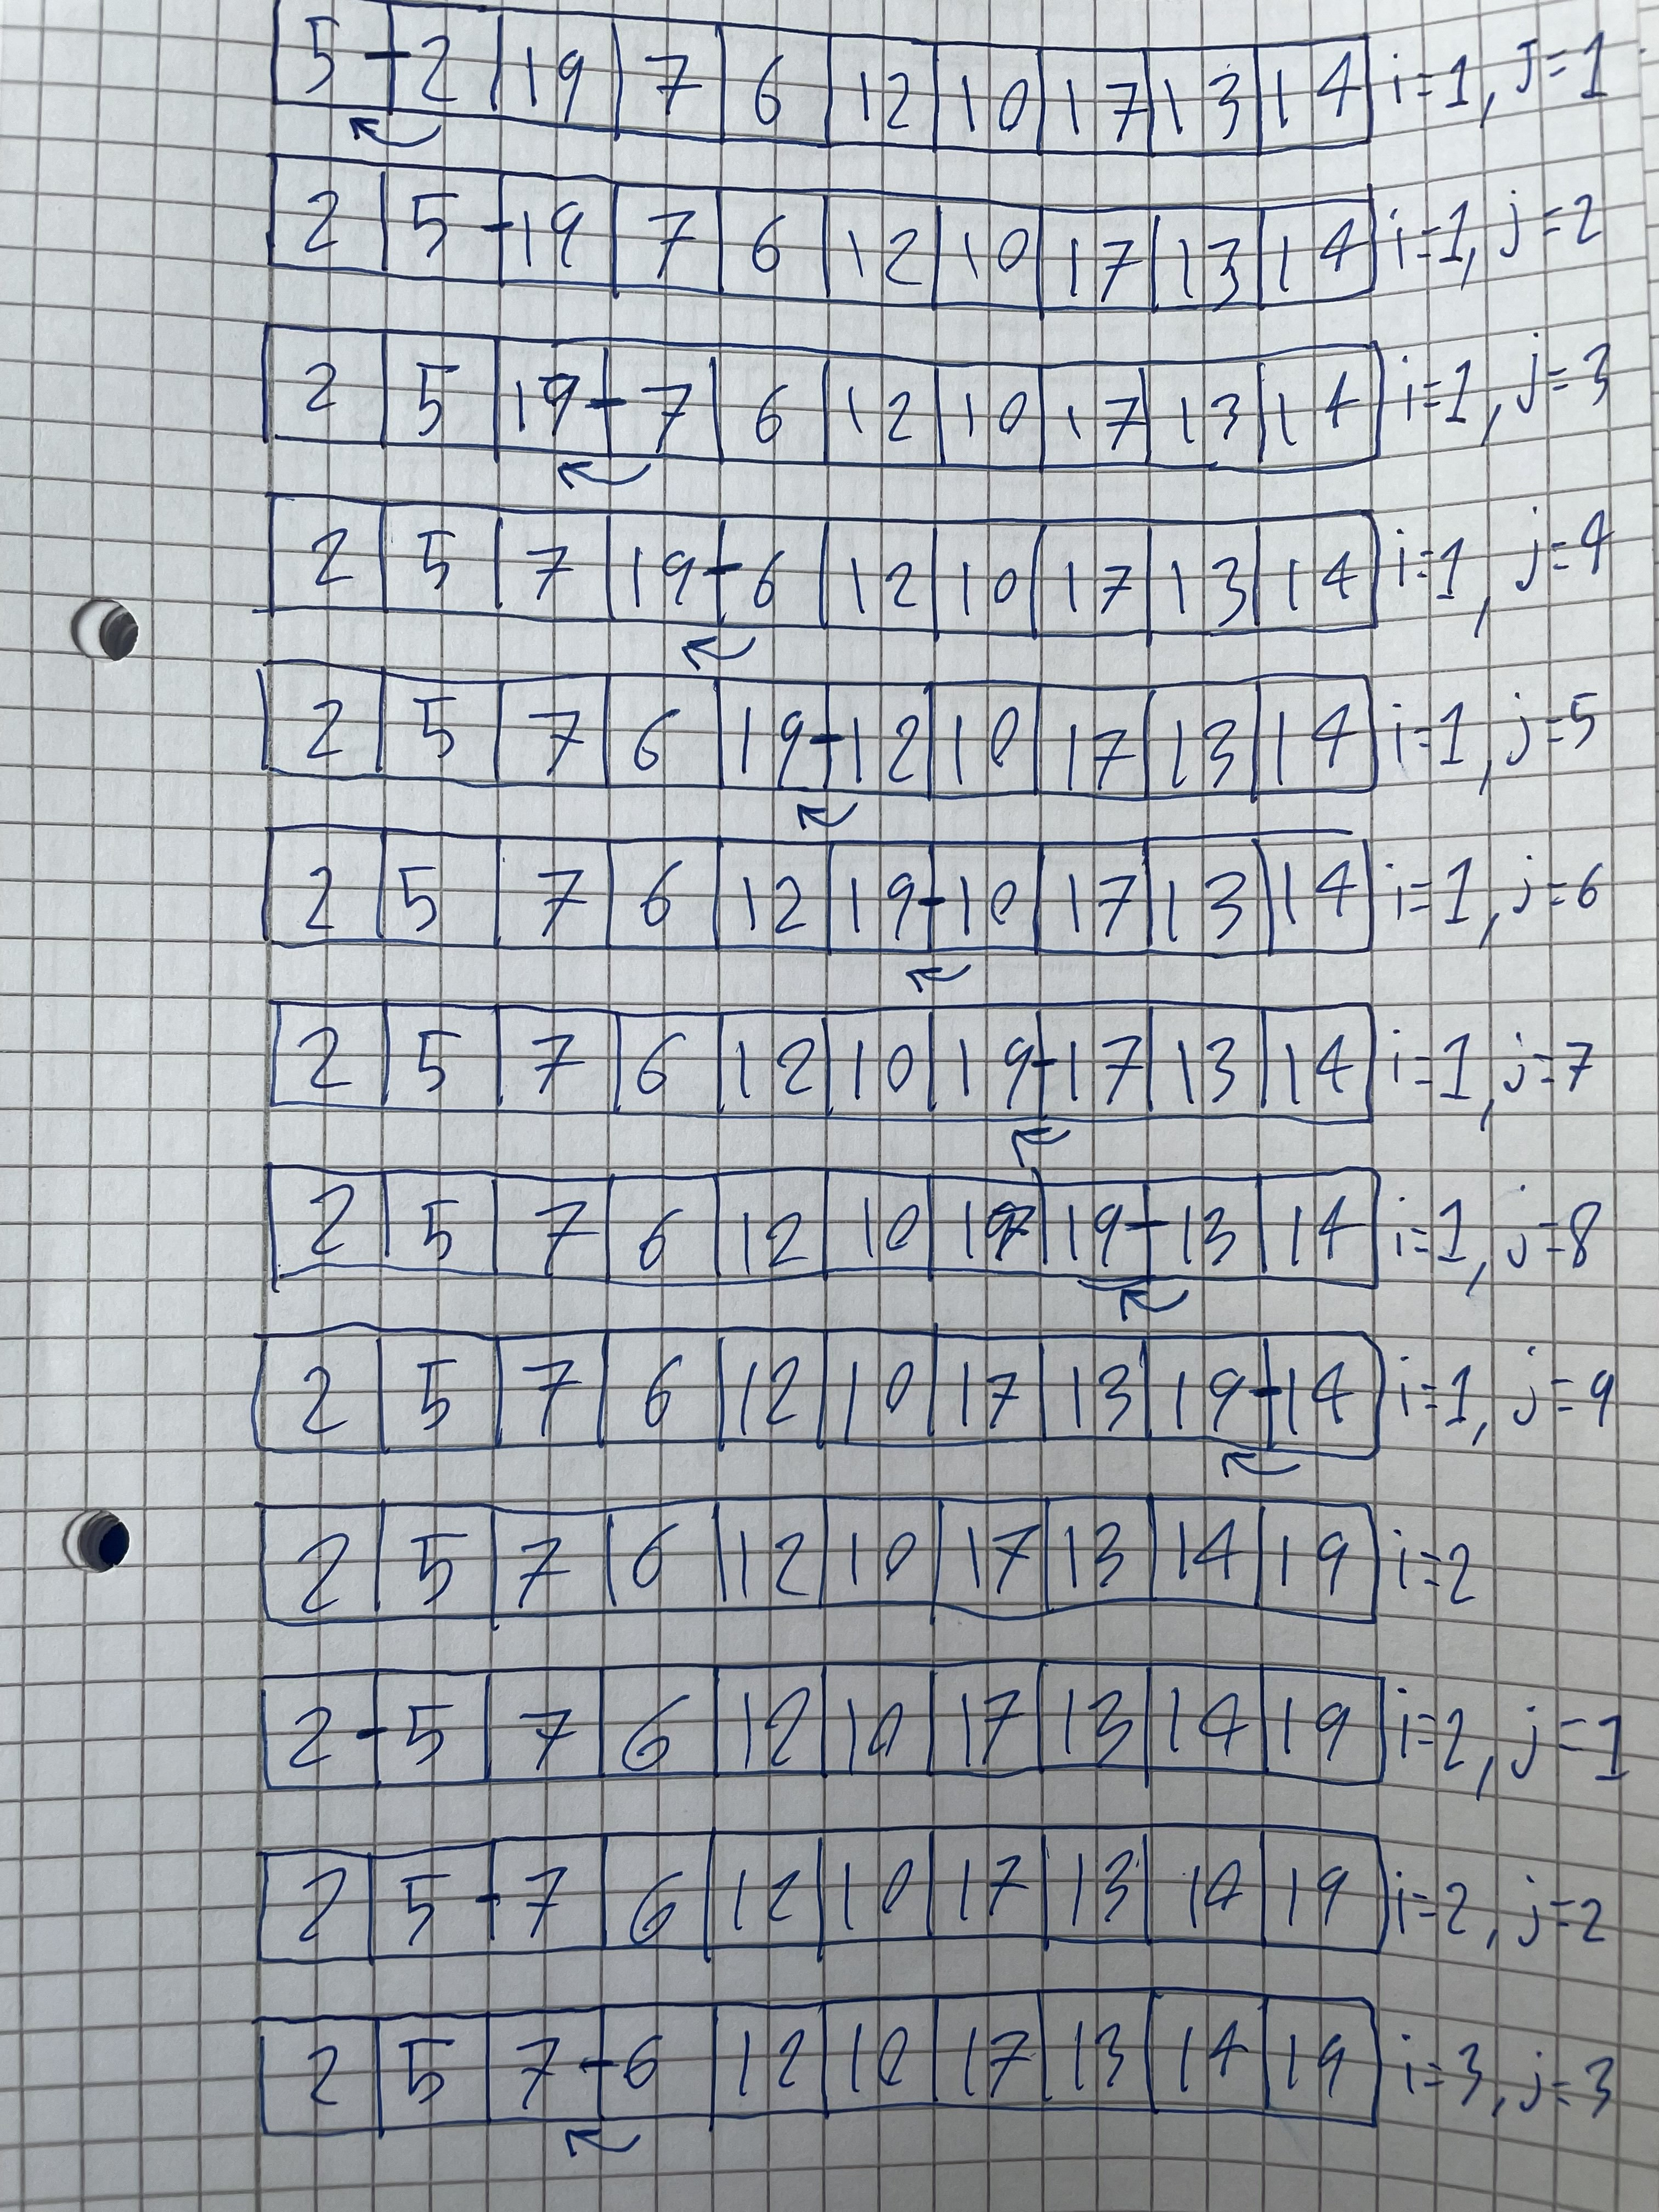
\includegraphics[scale=0.13]{IMG_2074.jpg}
\end{figure}
  
\clearpage

\begin{figure}[h]
    \centering
    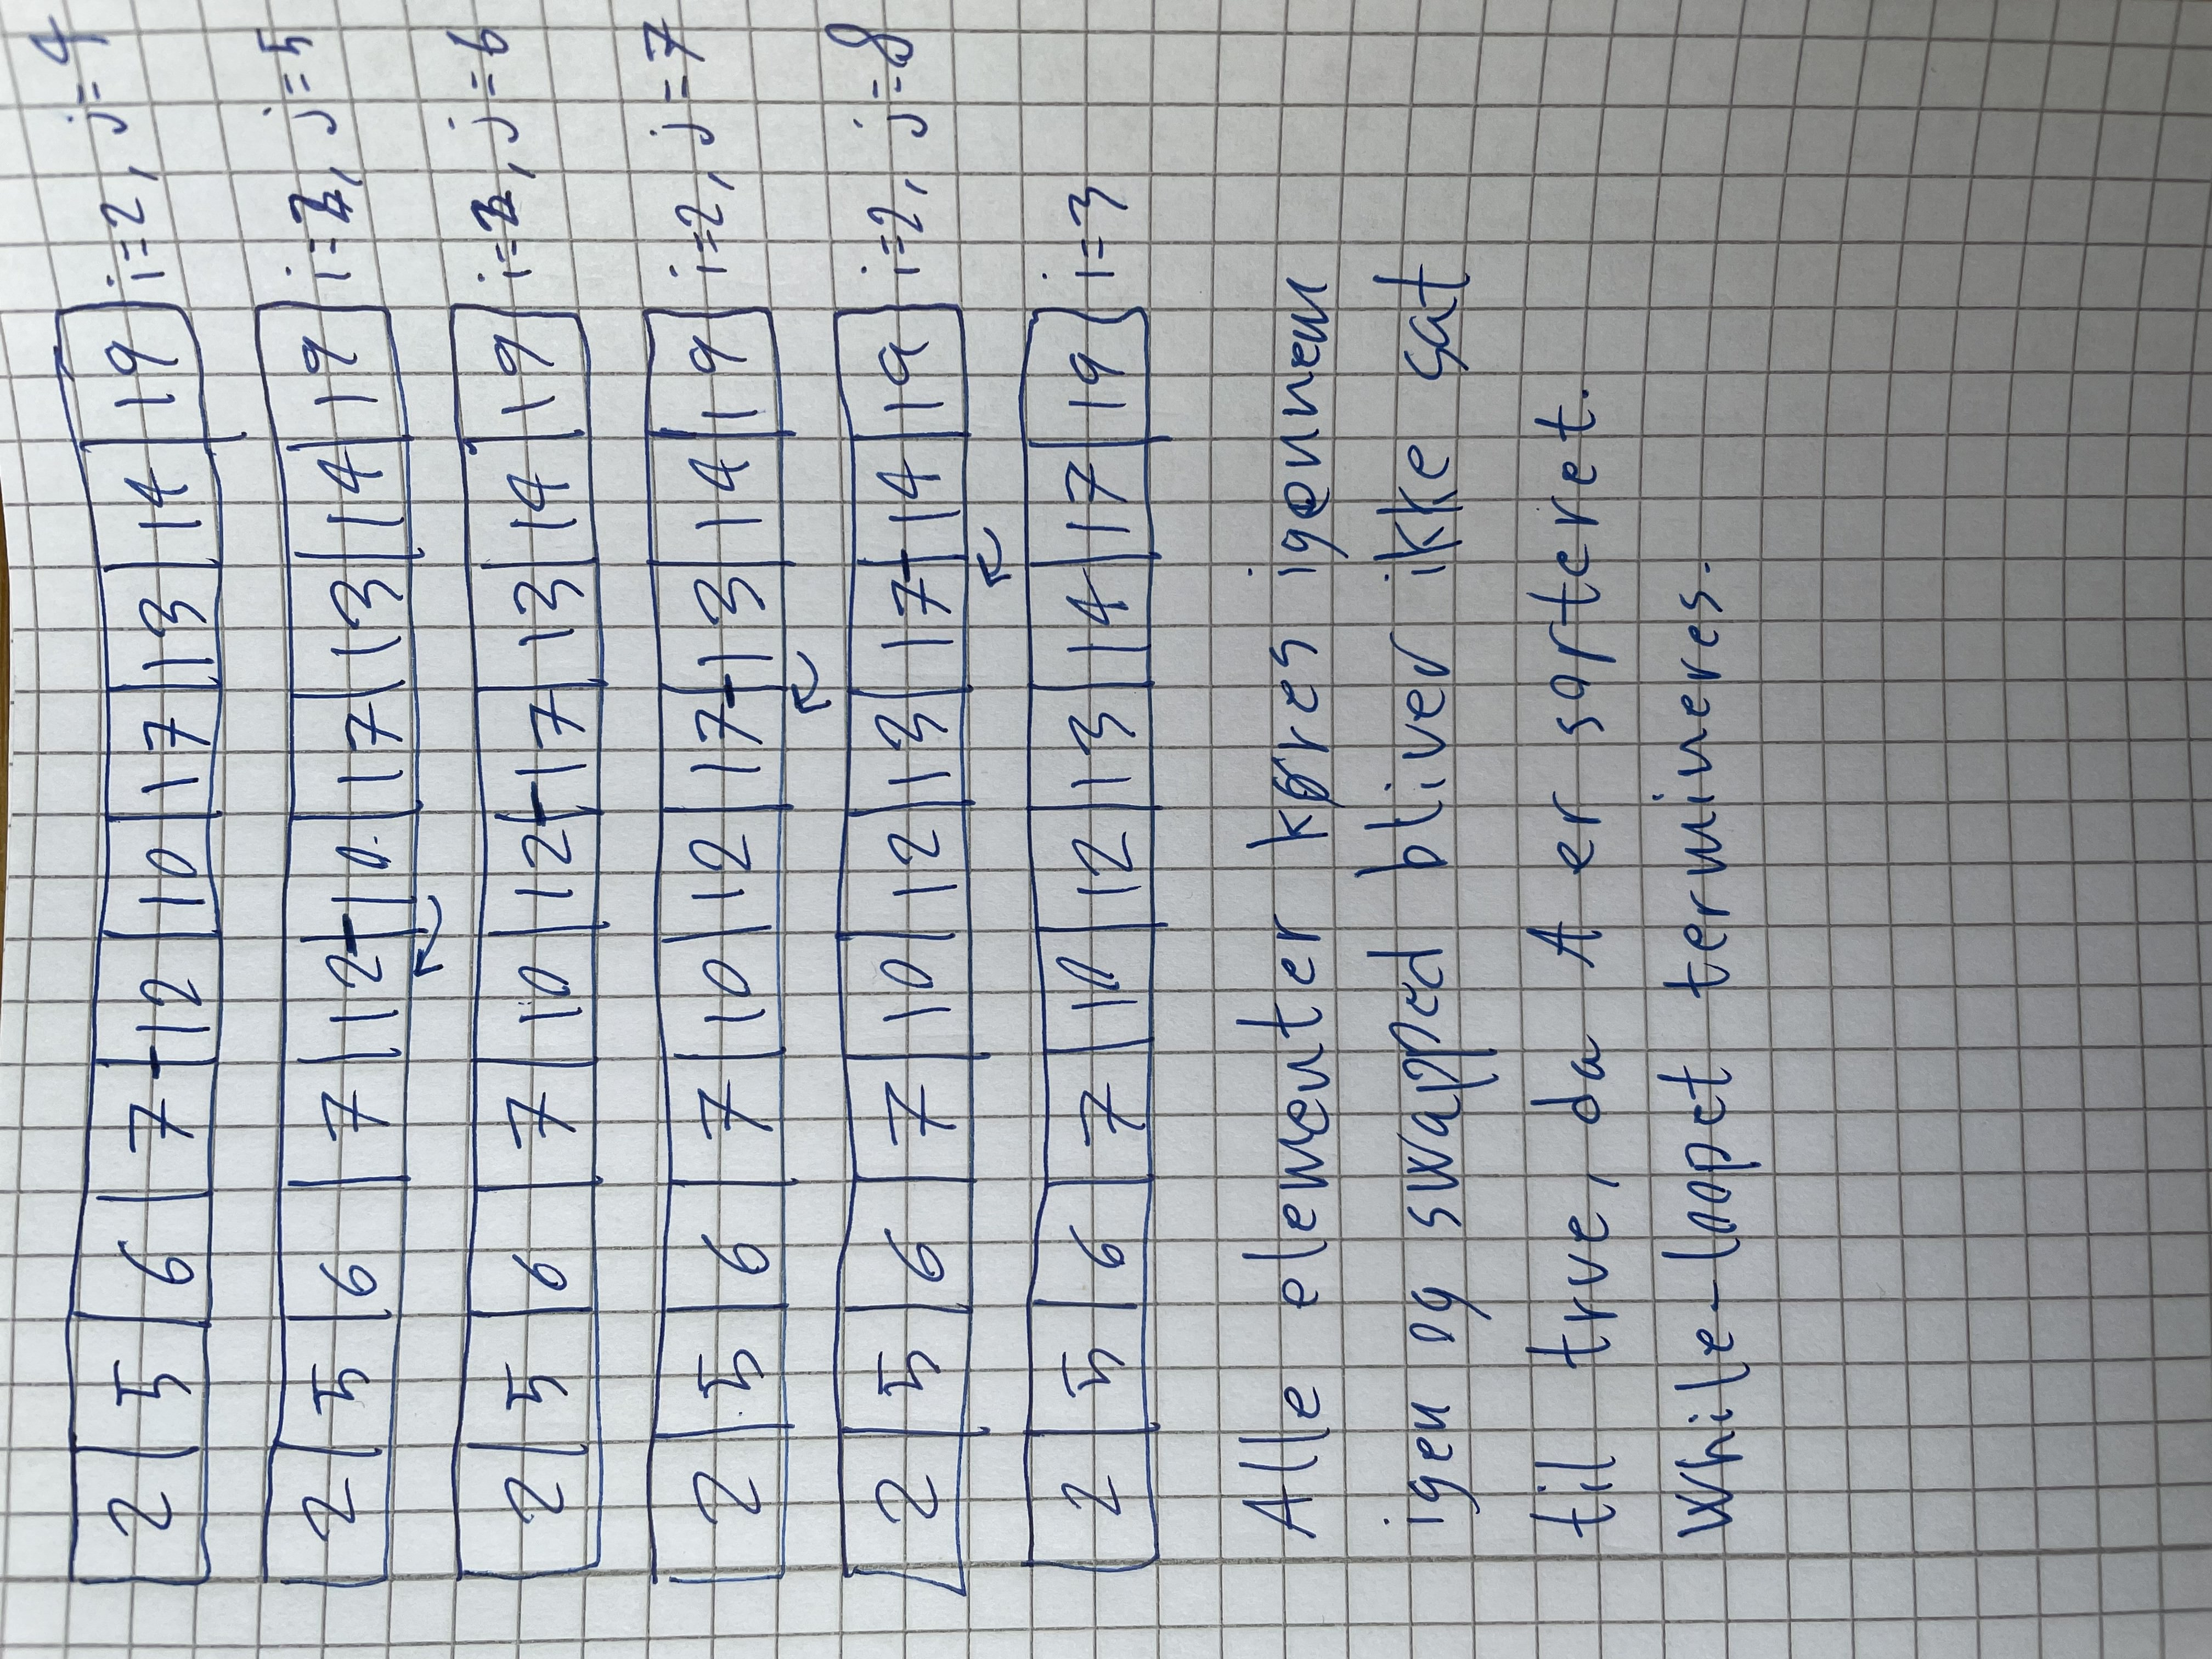
\includegraphics[scale=0.13, angle=-90]{IMG_2073.jpg}
\end{figure}

\clearpage

Vi kan argumentere for at algoritmet altid sorterer array'en korrekt, ved at analysere følgende:
\begin{itemize}
    \item Initialization: It is true prior to the first iteration of the loop.
    \item Maintenance: If it is true before an iteration of the loop, it remains true before the next iteration.
    \item Termination: The loop terminates, and when it terminates, the invariant - usually along with the reason that the loop terminated - gives us a useful property that helps show that the algorithm is correct.
\end{itemize}
Første iteration køres altid fra index $1\dots n$, da swapped er true, og for-loop'et kører optil $n$. Dette gøres på grund af, at for-loop'et kører til $size(A) - i$, hvor $i = 1$ og vi sammenligner elementer med $A[j] > A[j+1]$, hvor $j = i$.\\
Vi kan derfor konkludere, at vi efter første iteration, har det største element i index'et $n$ (sidste element).\\
Antag, at array'en ikke nu er sorteret, og at swapped nu er true, ellers vil vi terminere algoritmet, og arrayen er sorteret.\\
Vi nu ved, at det sidste element, er det største. I næste iteration køres while-loop'et nu på $i$ += $1$, og for-loop'et optil denne længden - $i$. Resultatet er igen, at array'en, er sorteret fra længen - $i$.\\ 
Således kører while-loop'et, og vi ved dermed, at array'en mindst er sorteret, fra index: (længden - $i$) til $n$.\\
\\
Lad os nu analysere time complexity'en af algoritmet.\\
I det værste tilfælde, køres for-loop'et $n$ gange, da det køres en grang for hvert element i array'en $A$. While-loopet køres også $n$ gange, da det iteres fra $1\dots size(A)$. For-loop'et findes inde i while-loop'et, hvilket giver os en worst case asympototic tim complexity på:\\
\[\sum_{j=1}^{n}j^2 = \dfrac{n(n+1)}{2} = O(n^2)\]
\centering \textit{Konstante led og led af lavere grad ignorares.}

\subsection[]{Run merge sort by hand on the array in (1) (as in the notes for the lectures). Show in every step of the algorithm what recursive calls are made and how the results from these recursive calls are combined, and make sure to explain the final (and most interesting) merge step carefully. (Any clear way of explaining is fine—you do not have to learn how to draw pictures in \LaTeX\ if you do not want to.)} 

\begin{figure}[h]
    \centering
    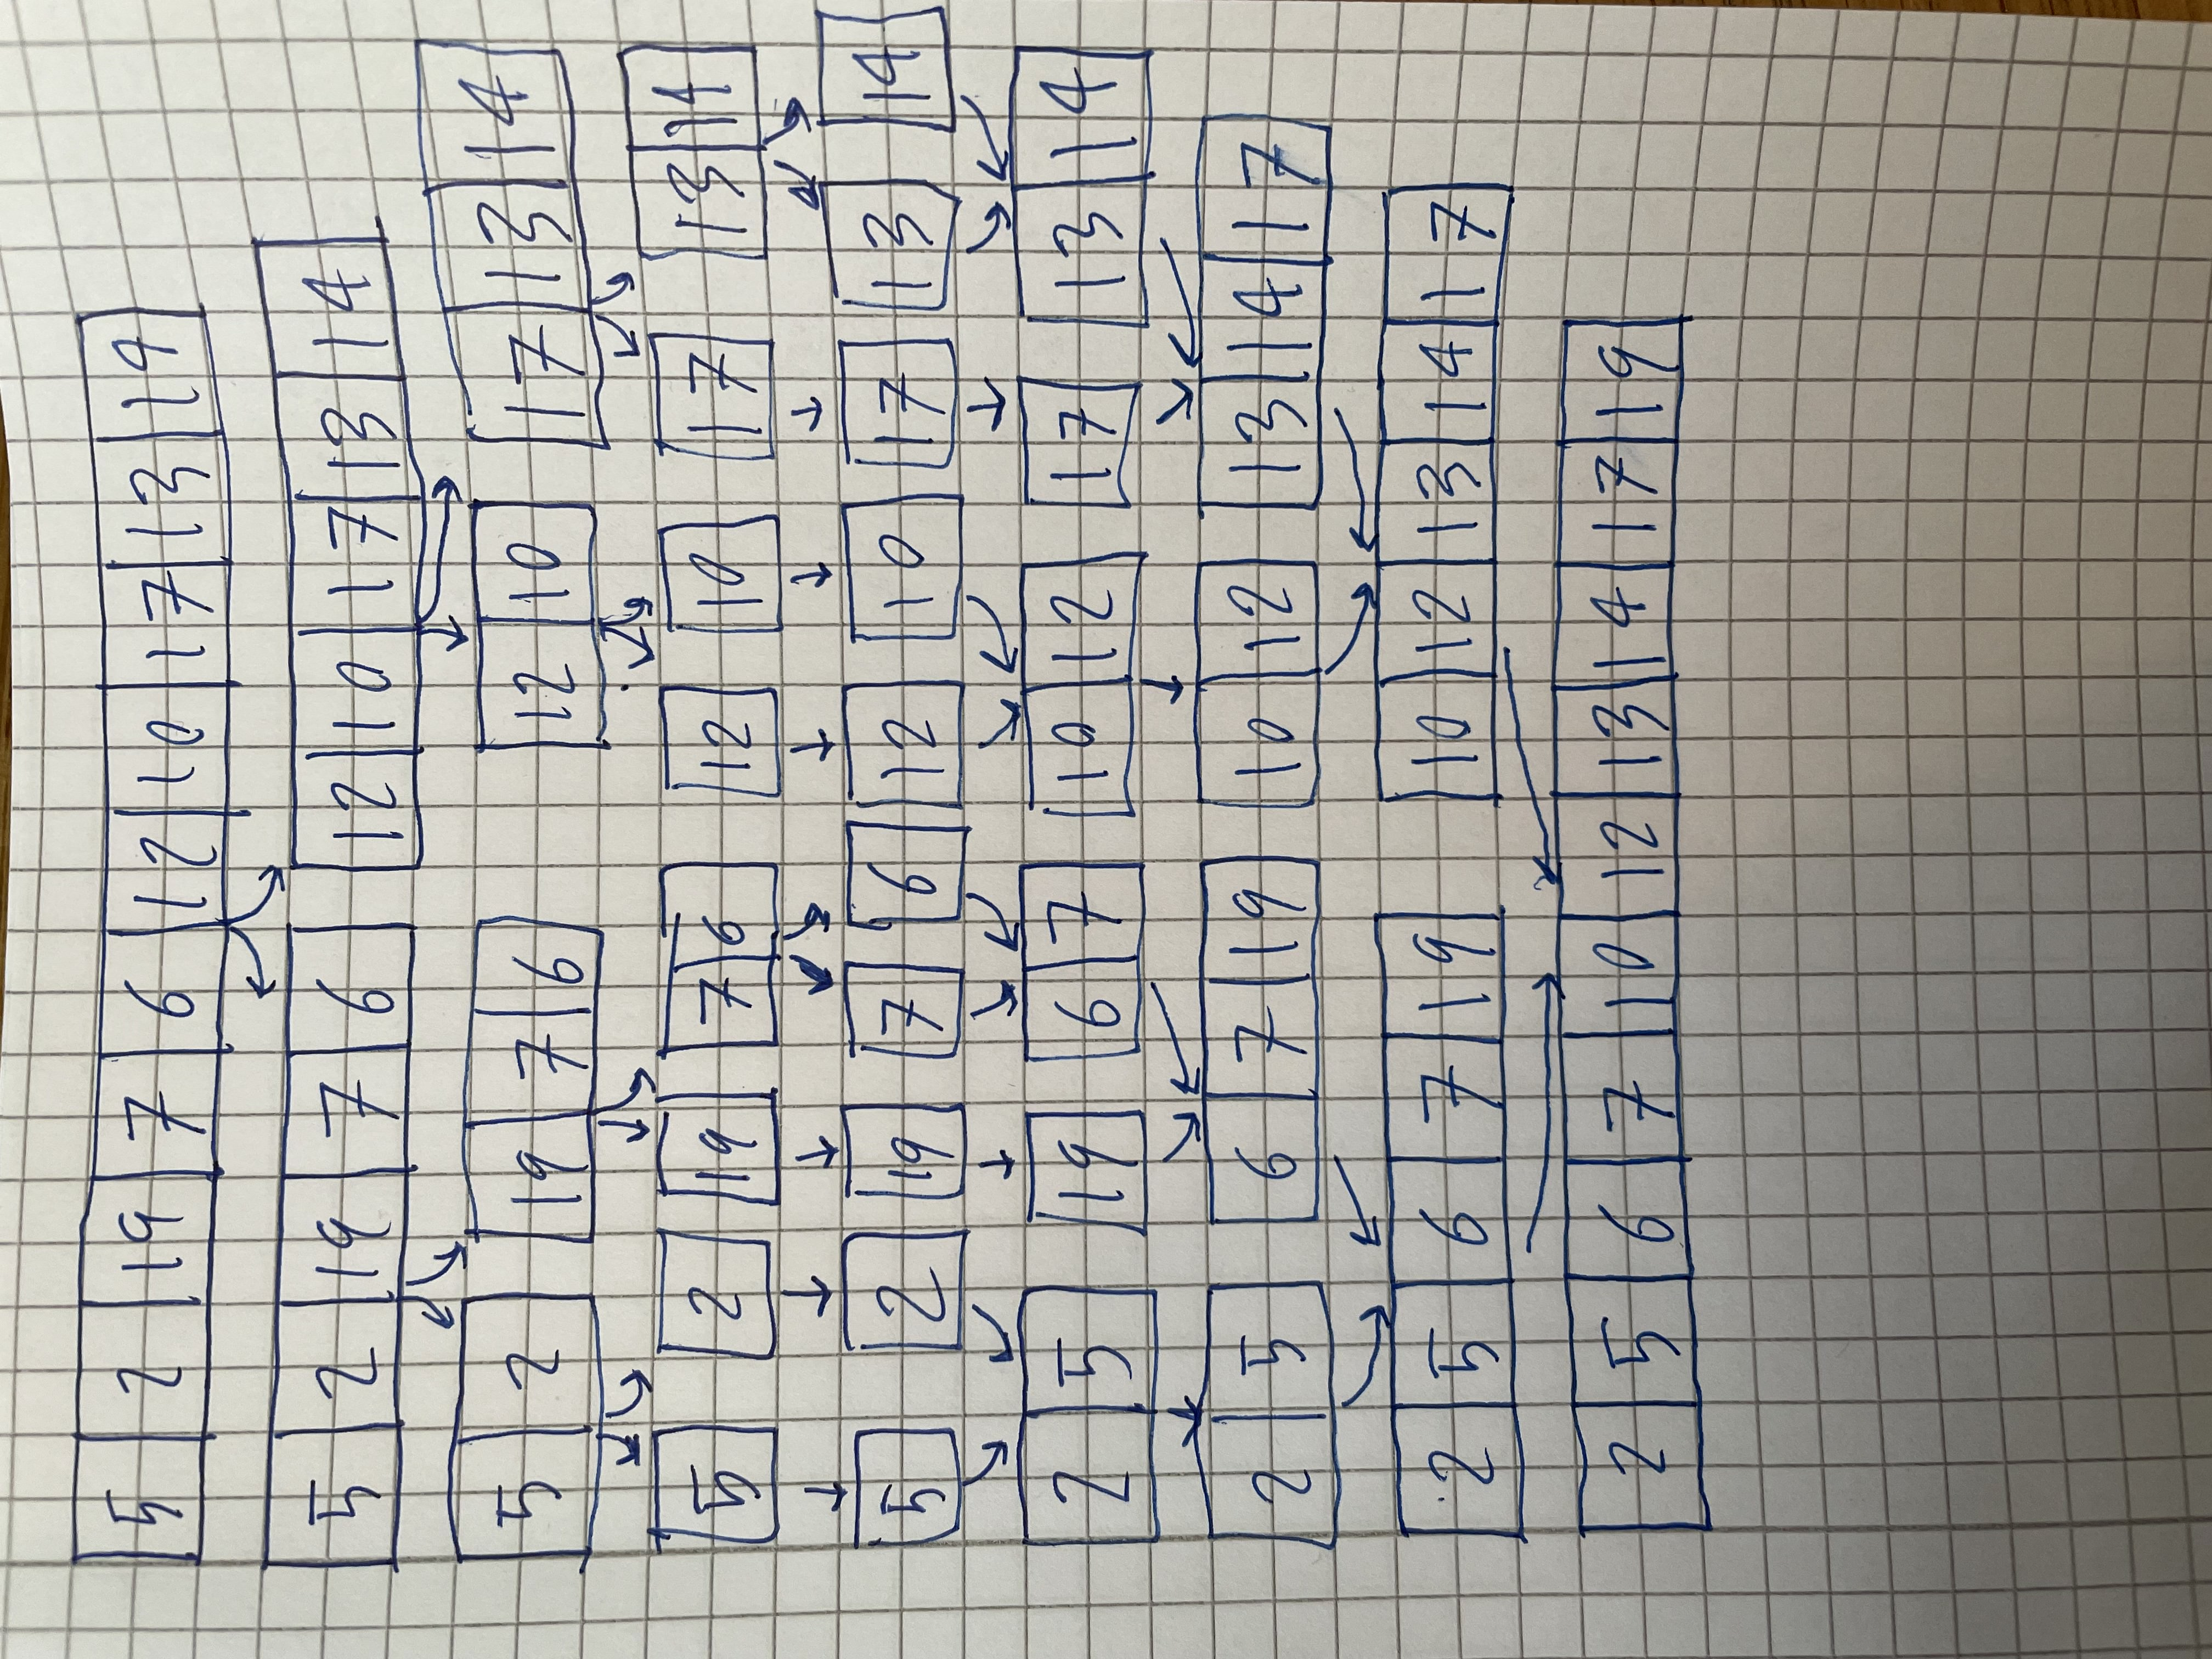
\includegraphics[scale=0.13, angle=-90]{IMG_2075.jpg}
\end{figure}

\clearpage

I sidste step, har vi to sorterede arrays:\\
\[[2, 5, 6, 7, 19]\] og \[[10, 12, 13, 14, 17]\] \\
Lad os kalde dem hhv. $L$ og $R$.\\
Vi sammenligner nu de første elementer i de to arrays:\\
\[L[1] \leq R[1]\]
Da $L[1] \leq R[1]$ kopirer vi dette element til A[1].\\
\[A = [2, 2, 19, 7, 6, 12, 10, 18, 13, 14]\]
Da det mindre element var I $L$ kigger vi nu på næste element i $L$:
\[L[2] \leq R[1]\]
Da $L[2] \leq R[1]$ kopirer vi dette element til A[2].\\
\[A = [2, 5, 19, 7, 6, 12, 10, 18, 13, 14]\]
Da det mindre element var I $L$ kigger vi nu på næste element i $L$:
\[\vdots\]
\[L[5] > R[5]\]
Da $L[5] > R[5]$ kopirer vi dette element til A[9].\\
\[A = [2, 5, 6, 7, 10, 12, 13, 14, 17, 14]\]
Til sidst bliver sidste element af $R$ kopieret til $A[10]$, da der ikke er flere elemnter i $L$.\\
Således ender vi med den sorterede array $A$:\\
\[A = [2, 5, 6, 7, 10, 12, 13, 14, 17, 19]\]

\subsection[]{Suppose that we are given another array $B$ of size $n$ that is already sorted in increasing order. How fast do the merge sort and optimized bubblesort algorithms run in this case? Is any of them asymptotically faster than the other as the size of the array $B$ grows?}



\subsection[]{Suppose that we are given a third array $C$ of size $n$ that is sorted in decreasing order, so that it needs to be reversed to be sorted in the order that we prefer, namely increasing. How fast do the merge sort and optimized bubblesort algorithms run in this case? Is any of them asymptotically faster than the other as the size of the array $C$ grows?}

\section[Question 2]{In 2021 DIKU celebrated its 50th anniversary with a lot of pomp, although slightly less emphasis was given to the fact that it was done one year late due to the Covid pandemic. Even less publicity was given to the public outreach day organized in F\ae lledsparken for school children by the Algorithms and Complexity Section as part of the anniversary, for reasons that might become clearer after you have studied the problems below.}

\subsection[]{In one of the events of the AC Section outreach day, Jakob had arranged so that 51 children were given brightly coloured balls, and were positioned in a field in such a way that all the pairwise distances between the children were distinct. The children were then asked to identify which other child was closest to them and, at a given signal, to throw their ball to this child (and hopefully also receive an incoming ball from somewhere). This turned out to be a public relations catastrophe. However, the children were positioned as described above, every time at least one child ended up without a ball (but instead with tears in the eyes). This did not at all generate the goodwill DIKU was hoping for. What went wrong? Was Jakob just immensely unlucky? Or can you prove mathematically that it was unavoidable that at least one child would end up without a ball? Would this have been different if Jakob had not insisted on 51 children, but had accepted the proposal by his colleagues to have 50 children? Or if not all distances would have had to be different?}

\begin{figure}[h]
    \centering
    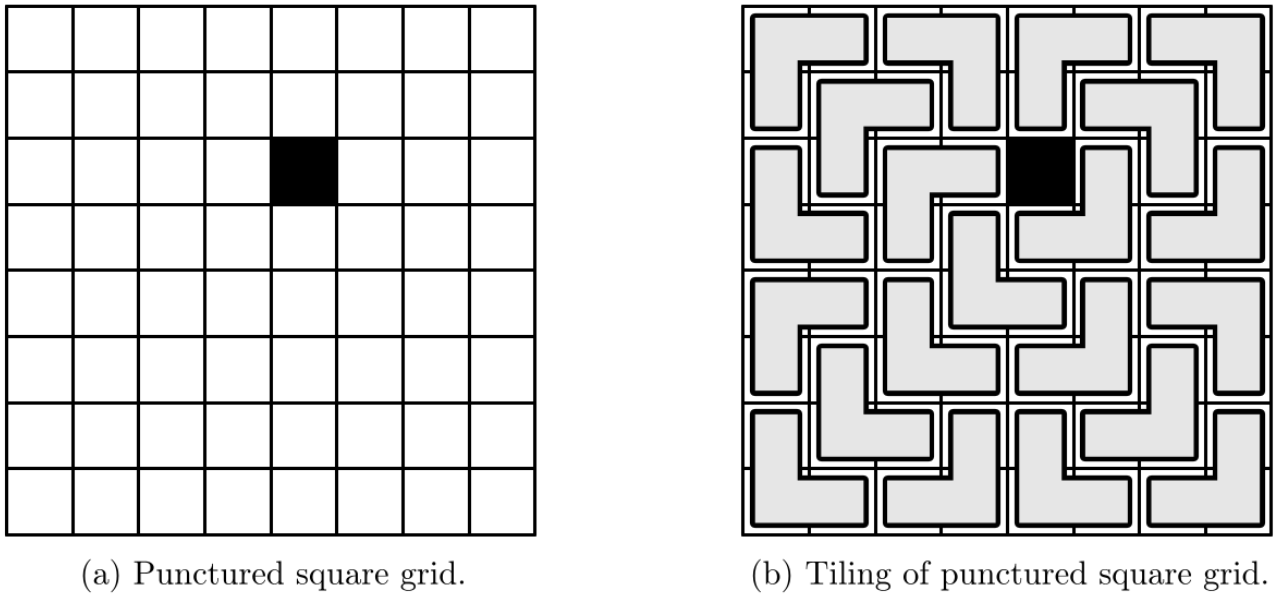
\includegraphics[scale=0.5]{figur.png}
\end{figure}

\subsection[]{In another event, Jakob built a 5-kilometre car track across the park. On this track, 51 electric cars were placed at random locations (but all pointing in the same direction clockwise around the circuit). One car battery was sufficient for exactly one full lap if charged to 100\% capacity. However, instead the batteries of all the cars were charged partially in such a way that the total charge of all the batteries together was sufficient for one car to travel exactly the full distance of 5 kilometres. After this, the batteries were distributed to the cars in some random way. The children were given the challenge to start driving one car in such a way that one full lap of the track would covered. The rules were that if one car travelled far enough to bump into the rear of the car in front, then this next car could continue, and also the battery from the car behind could be shifted to the car in front so that the front car could use any remaining charge (and similarly for any other batteries picked up along the way). If, however, a car would run out of batteries before reaching the car in front, or before the full lap was completed by all the cars together, this was a failure. This event went slightly better, in that the children were able to figure out a solution to the challenge most of the time. Jakob prided himself with that this was thanks to the fact that he had given the friendly advice, to avoid more embarrassment as in Problem 2a, that a good strategy was to start with the car with the most charge in its battery. Were the children just lucky this time, or can you prove that there is always a solution to this challenge? And is it a good idea to follow Jakob’s advice, or does it seem more likely that the children figured out something smarter?}

\subsection[]{In the final event of the day, a big $2^n$-by-$2^n$ grid was constructed, after which one cell in the grid was removed by placing a black square on it as illustrated in Figure 1a. The children were then given the task to cover all the other cells in the grid by placing L-shaped tiles in such a way that every cell was covered exactly once, and nothing outside of the grid was covered, as shown in Figure 1b. By now the children were fairly fed up with these strange games, however, and Jakob’s colleagues also started getting a bit annoyed, wondering if the strange shape of the tiles was somehow a not-so-subtle attempt to push for a competing foreign university at the other side of the Øresund strait instead, and the day did not end on a festive note at all. Disregarding this unfortunate turn of events, can you prove that it is actually true that for any $2^n$-by-$2^n$ grid, regardless of how it is punctured by removing a cell, it is always possible to tile the rest of the grid with L-shaped tiles?}

\end{document}